\documentclass[border=10pt]{standalone}
\usepackage{tikz}
\usetikzlibrary{arrows.meta, positioning, calc}

\begin{document}
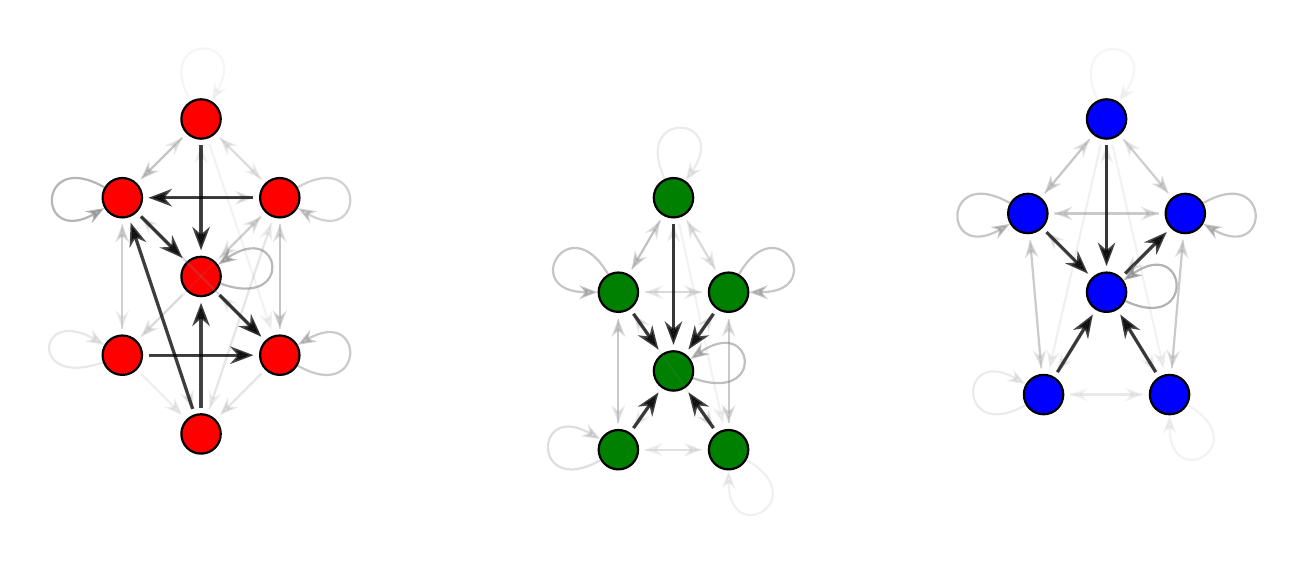
\begin{tikzpicture}[
    node/.style={circle, draw=black, thick, minimum size=5mm, inner sep=0pt},
    rednode/.style={node, fill=red},
    greennode/.style={node, fill=green!50!black},
    bluenode/.style={node, fill=blue},
    grayedge/.style={->, gray, thick, >=Stealth, shorten >=2pt, shorten <=2pt},
    blackedge/.style={->, black, very thick, >=Stealth, shorten >=2pt, shorten <=2pt},
    loop/.style={->, gray, thick, >=Stealth, looseness=8, min distance=10mm}
]

% RED GRAPH (Left)
\begin{scope}[xshift=0cm]
    % Nodes
    \node[rednode] (r1) at (0, 3) {};
    \node[rednode] (r2) at (-1, 2) {};
    \node[rednode] (r3) at (1, 2) {};
    \node[rednode] (r4) at (0, 1) {};
    \node[rednode] (r5) at (-1, 0) {};
    \node[rednode] (r6) at (1, 0) {};
    \node[rednode] (r7) at (0, -1) {};
    
    % Varied faint directed edges
    \draw[grayedge, opacity=.35] (r1) -- (r2);
    \draw[grayedge, opacity=.12] (r1) -- (r3);
    \draw[grayedge, opacity=.30] (r1) -- (r4);
    \draw[grayedge, opacity=.10] (r1) -- (r6);
    \draw[grayedge, opacity=.16] (r2) -- (r1);
    \draw[grayedge, opacity=.22] (r2) -- (r3);
    \draw[grayedge, opacity=.24] (r2) -- (r4);
    \draw[grayedge, opacity=.13] (r2) -- (r5);
    \draw[grayedge, opacity=.28] (r2) -- (r6);
    \draw[grayedge, opacity=.18] (r2) -- (r7);
    \draw[grayedge, opacity=.16] (r3) -- (r1);
    \draw[grayedge, opacity=.28] (r3) -- (r2);
    \draw[grayedge, opacity=.20] (r3) -- (r4);
    \draw[grayedge, opacity=.30] (r3) -- (r6);
    \draw[grayedge, opacity=.10] (r3) -- (r7);
    \draw[grayedge, opacity=.10] (r4) -- (r1);
    \draw[grayedge, opacity=.15] (r4) -- (r2);
    \draw[grayedge, opacity=.13] (r4) -- (r3);
    \draw[grayedge, opacity=.20] (r4) -- (r5);
    \draw[grayedge, opacity=.32] (r4) -- (r6);
    \draw[grayedge, opacity=.28] (r5) -- (r2);
    \draw[grayedge, opacity=.11] (r5) -- (r3);
    \draw[grayedge, opacity=.35] (r5) -- (r6);
    \draw[grayedge, opacity=.14] (r5) -- (r7);
    \draw[grayedge, opacity=.22] (r6) -- (r3);
    \draw[grayedge, opacity=.12] (r6) -- (r4);
    \draw[grayedge, opacity=.20] (r6) -- (r7);
    \draw[grayedge, opacity=.16] (r7) -- (r2);
    \draw[grayedge, opacity=.11] (r7) -- (r3);
    \draw[grayedge, opacity=.26] (r7) -- (r4);
    
    % Prominent directed edges
    \draw[blackedge, opacity=.72] (r3) -- (r2);
    \draw[blackedge, opacity=.72] (r1) -- (r4);
    \draw[blackedge, opacity=.72] (r2) -- (r4);
    \draw[blackedge, opacity=.72] (r4) -- (r6);
    \draw[blackedge, opacity=.72] (r5) -- (r6);
    \draw[blackedge, opacity=.72] (r7) -- (r4);
    \draw[blackedge, opacity=.72] (r7) -- (r2);
    
    % Self-loops
    \draw[loop, opacity=.08] (r1) to[out=120, in=60] (r1);
    \draw[loop, opacity=.58] (r2) to[out=150, in=210] (r2);
    \draw[loop, opacity=.36] (r3) to[out=30, in=-30] (r3);
    \draw[loop, opacity=.55] (r4) to[out=-20, in=35, looseness=7] (r4);
    \draw[loop, opacity=.18] (r5) to[out=200, in=150] (r5);
    \draw[loop, opacity=.42] (r6) to[out=-30, in=30] (r6);
\end{scope}

% GREEN GRAPH (Middle)
\begin{scope}[xshift=6cm]
    % Nodes
    \node[greennode] (g1) at (0, 2) {};
    \node[greennode] (g2) at (-0.7, 0.8) {};
    \node[greennode] (g3) at (0.7, 0.8) {};
    \node[greennode] (g4) at (0, -0.2) {};
    \node[greennode] (g5) at (-0.7, -1.2) {};
    \node[greennode] (g6) at (0.7, -1.2) {};
    
    % Varied faint directed edges
    \draw[grayedge, opacity=.32] (g1) -- (g2);
    \draw[grayedge, opacity=.16] (g1) -- (g3);
    \draw[grayedge, opacity=.35] (g1) -- (g4);
    \draw[grayedge, opacity=.10] (g1) -- (g6);
    \draw[grayedge, opacity=.22] (g2) -- (g1);
    \draw[grayedge, opacity=.18] (g2) -- (g3);
    \draw[grayedge, opacity=.25] (g2) -- (g4);
    \draw[grayedge, opacity=.18] (g2) -- (g5);
    \draw[grayedge, opacity=.12] (g2) -- (g6);
    \draw[grayedge, opacity=.16] (g3) -- (g1);
    \draw[grayedge, opacity=.14] (g3) -- (g2);
    \draw[grayedge, opacity=.24] (g3) -- (g4);
    \draw[grayedge, opacity=.25] (g3) -- (g6);
    \draw[grayedge, opacity=.13] (g4) -- (g1);
    \draw[grayedge, opacity=.20] (g4) -- (g2);
    \draw[grayedge, opacity=.18] (g4) -- (g3);
    \draw[grayedge, opacity=.12] (g4) -- (g5);
    \draw[grayedge, opacity=.13] (g4) -- (g6);
    \draw[grayedge, opacity=.30] (g5) -- (g2);
    \draw[grayedge, opacity=.28] (g5) -- (g4);
    \draw[grayedge, opacity=.15] (g5) -- (g6);
    \draw[grayedge, opacity=.22] (g6) -- (g3);
    \draw[grayedge, opacity=.26] (g6) -- (g4);
    \draw[grayedge, opacity=.10] (g6) -- (g5);
    
    % Prominent directed edges
    \draw[blackedge, opacity=.72] (g2) -- (g4);
    \draw[blackedge, opacity=.72] (g3) -- (g4);
    \draw[blackedge, opacity=.72] (g1) -- (g4);
    \draw[blackedge, opacity=.72] (g5) -- (g4);
    \draw[blackedge, opacity=.72] (g6) -- (g4);
    
    % Self-loops
    \draw[loop, opacity=.16] (g1) to[out=115, in=55] (g1);
    \draw[loop, opacity=.45] (g2) to[out=120, in=180] (g2);
    \draw[loop, opacity=.45] (g3) to[out=60, in=0] (g3);
    \draw[loop, opacity=.50] (g4) to[out=-20, in=35, looseness=7] (g4);
    \draw[loop, opacity=.26] (g5) to[out=210, in=150] (g5);
    \draw[loop, opacity=.12] (g6) to[out=-30, in=-90, looseness=7] (g6);
\end{scope}

% BLUE GRAPH (Right)
\begin{scope}[xshift=11.5cm]
    % Nodes
    \node[bluenode] (b1) at (0, 3) {};
    \node[bluenode] (b2) at (-1, 1.8) {};
    \node[bluenode] (b3) at (1, 1.8) {};
    \node[bluenode] (b4) at (0, 0.8) {};
    \node[bluenode] (b5) at (-0.8, -0.5) {};
    \node[bluenode] (b6) at (0.8, -0.5) {};
    
    % Varied faint directed edges
    \draw[grayedge, opacity=.30] (b1) -- (b2);
    \draw[grayedge, opacity=.28] (b1) -- (b3);
    \draw[grayedge, opacity=.35] (b1) -- (b4);
    \draw[grayedge, opacity=.12] (b1) -- (b5);
    \draw[grayedge, opacity=.10] (b1) -- (b6);
    \draw[grayedge, opacity=.20] (b2) -- (b1);
    \draw[grayedge, opacity=.22] (b2) -- (b3);
    \draw[grayedge, opacity=.25] (b2) -- (b4);
    \draw[grayedge, opacity=.18] (b2) -- (b5);
    \draw[grayedge, opacity=.14] (b3) -- (b1);
    \draw[grayedge, opacity=.25] (b3) -- (b2);
    \draw[grayedge, opacity=.20] (b3) -- (b4);
    \draw[grayedge, opacity=.22] (b3) -- (b6);
    \draw[grayedge, opacity=.12] (b4) -- (b1);
    \draw[grayedge, opacity=.18] (b4) -- (b2);
    \draw[grayedge, opacity=.16] (b4) -- (b3);
    \draw[grayedge, opacity=.13] (b4) -- (b5);
    \draw[grayedge, opacity=.13] (b4) -- (b6);
    \draw[grayedge, opacity=.28] (b5) -- (b2);
    \draw[grayedge, opacity=.30] (b5) -- (b4);
    \draw[grayedge, opacity=.10] (b5) -- (b6);
    \draw[grayedge, opacity=.25] (b6) -- (b3);
    \draw[grayedge, opacity=.30] (b6) -- (b4);
    \draw[grayedge, opacity=.08] (b6) -- (b5);
    
    % Prominent directed edges
    \draw[blackedge, opacity=.72] (b2) -- (b4);
    \draw[blackedge, opacity=.72] (b4) -- (b3);
    \draw[blackedge, opacity=.72] (b1) -- (b4);
    \draw[blackedge, opacity=.72] (b5) -- (b4);
    \draw[blackedge, opacity=.72] (b6) -- (b4);
    
    % Self-loops
    \draw[loop, opacity=.08] (b1) to[out=115, in=55] (b1);
    \draw[loop, opacity=.45] (b2) to[out=150, in=210] (b2);
    \draw[loop, opacity=.45] (b3) to[out=30, in=-30] (b3);
    \draw[loop, opacity=.60] (b4) to[out=-25, in=35, looseness=7] (b4);
    \draw[loop, opacity=.16] (b5) to[out=210, in=150] (b5);
    \draw[loop, opacity=.10] (b6) to[out=-30, in=-90, looseness=7] (b6);
\end{scope}

\end{tikzpicture}
\end{document}
